\documentclass[aps,prb,twocolumn,
	groupedaddress,superscriptaddress,
	amsfonts,amssymb,amsmath,floatfix,
	citeautoscript]{revtex4-1}

\usepackage{graphicx}
\usepackage[centering,hmargin=20mm,tmargin=30mm,bmargin=25mm]{geometry}
\usepackage{multirow}
\usepackage{newtxtext}
\usepackage[cmintegrals]{newtxmath}

%----- References -----
\usepackage{xcolor}
\usepackage{hyperref}
\hypersetup{colorlinks,
	linkcolor={blue!75!black!80!yellow},
	citecolor={blue!75!black!80!yellow},
	urlcolor={blue!75!black!80!yellow}
}

%----- Captions in sans font -----
\makeatletter
\renewcommand\@make@capt@title[2]{%
	\@ifx@empty\float@link{\@firstofone}{\expandafter\href\expandafter{\float@link}}%
	\sffamily{\textbf{#1}}\@caption@fignum@sep#2
}%
\renewcommand\figurename{Fig.}
\makeatother

\thickmuskip=5mu plus 2mu minus 1mu  %binary relations (default, 5mu plus 5mu)
\medmuskip=4mu plus 2mu minus 2mu    %binary operations (default, 4mu plus 2mu minus 4mu)

\frenchspacing %Ensure that revTeX does not do "double spaces" after punctuation

\renewcommand{\Im}{\operatorname{Im}}
\renewcommand{\Re}{\operatorname{Re}}
\newcommand{\sub}[1]{\ensuremath{_{\textrm{#1}}}} %Upright multi-character subscript
\newcommand{\super}[1]{\ensuremath{^{\textrm{#1}}}} %Upright multi-character superscript

\newcommand{\HarvardSEAS}{John A. Paulson School of Engineering and Applied Sciences, Harvard University, Cambridge, MA, USA}
\newcommand{\MITPhy}{Department of Physics, Massachusetts Institute of Technology, Cambridge, MA, USA}

%\usepackage[usenames]{color}
%\newcommand{\edited}[1]{{\color{red} #1}}

\begin{document}

\title{Variational theory of the ground state of cavity quantum electrodynamics}

\author{Nicholas Rivera$^\perp$}\email{nrivera@seas.harvard.edu}\affiliation{\HarvardSEAS}\affiliation{\MITPhy}
\author{Johannes Flick}\email{flick@g.harvard.edu}\affiliation{\HarvardSEAS}
\author{Prineha Narang}\email{prineha@seas.harvard.edu}\affiliation{\HarvardSEAS}


\date{\today}

\begin{abstract}

\end{abstract}

\maketitle


\section{Variational ansatz}

\subsection{Concept: Effectively non-interacting matter and photon systems}
\begin{figure*}[t]
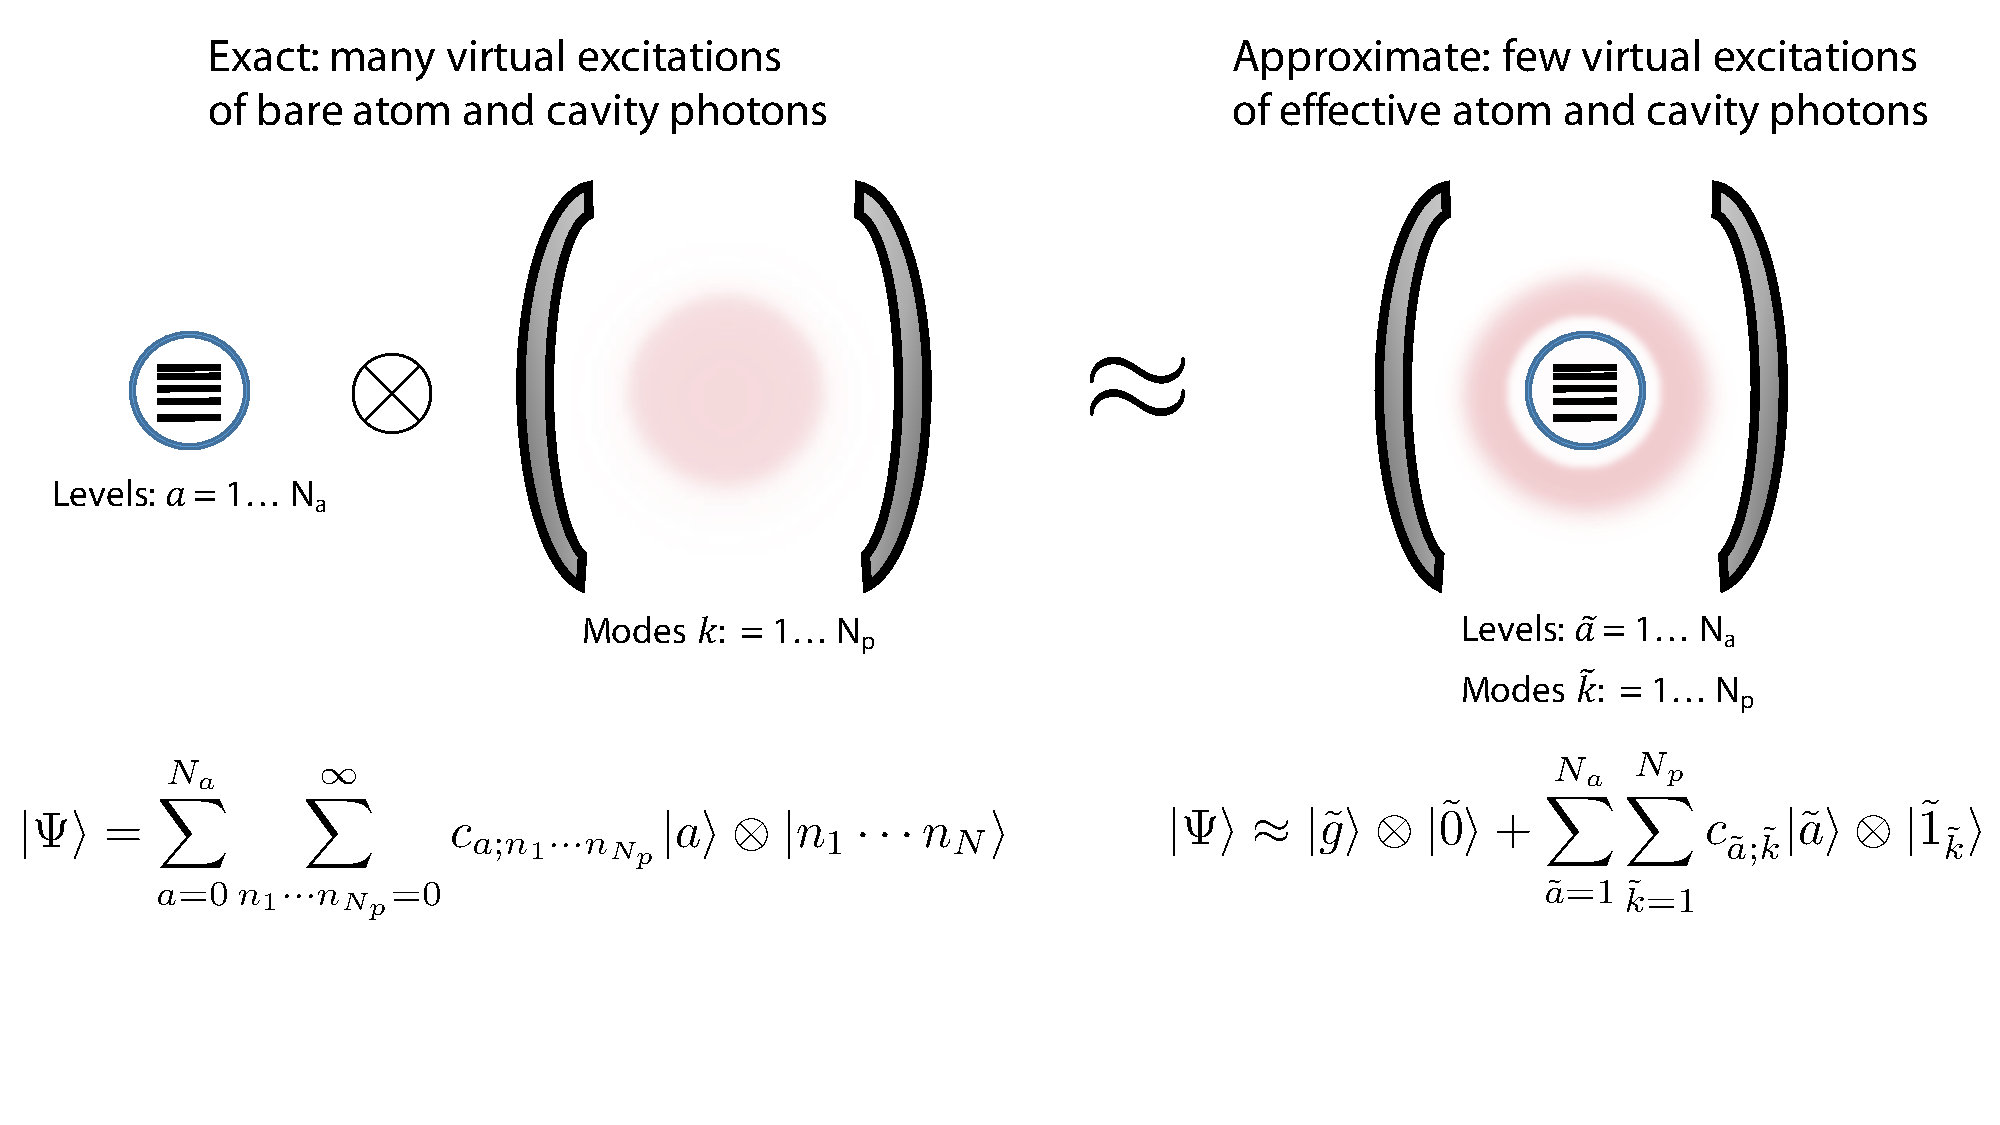
\includegraphics[width=18cm]{conceptfigure.pdf}
\caption{\textbf{Ground-state ansatz applied to matter in a cavity: effectively decoupled matter and photons.} .}
\label{fig:ansatz}
\end{figure*}

\subsection{Correlation corrections coming from virtual matter and photon quasiparticles}

\section{Application to a multi-level system coupled to a multi-mode cavity}

\section{Outlook}



\section{Acknowledgements}
% Pri, Johannes: Please insert any other relevant acknowledgement information here!
N. R. and J. C. recognize the support of the DOE Computational Science Graduate Fellowship (CSGF) fellowship no.  DE-FG02-97ER25308. P. N. acknowledges start-up funding from the Harvard John A. Paulson School of Engineering and Applied Sciences. %The authors thank XXXX for helpful discussions. Tentatively Joel Yuen Zhou and Javier Aizpurua.

\bibliographystyle{apsrev4-1}
\bibliography{references}

\end{document}
